% \documentclass{article}

% \usepackage{iclr2026_conference,times}
% \usepackage{lipsum}
% \usepackage{graphicx,subfig,subfigure}
% \usepackage{wrapfig,lipsum,booktabs}

% \usepackage{tikz}
% \usepackage{comment}
% \usepackage{amsmath,amssymb} % define this before the line numbering.
% \usepackage{bm}
% \usepackage{gensymb}
% \usepackage{subcaption}

% \usepackage{graphicx}
% \usepackage[group-separator={,}]{siunitx}
% \usepackage{multirow}
% \usepackage{placeins}
% \usepackage{enumitem}
% \usepackage{paralist}

% \usepackage[table,xcdraw]{xcolor}
%\usepackage{overpic}
% \usepackage{array}
% \usepackage{xfrac}

% \usepackage[utf8]{inputenc} % allow utf-8 input
% \usepackage[T1]{fontenc}    % use 8-bit T1 fonts
%\usepackage{hyperref}       % hyperlinks
% \usepackage{url}            % simple URL typesetting
% \usepackage{booktabs}       % professional-quality tables
% \usepackage{amsfonts}       % blackboard math symbols
% \usepackage{nicefrac}       % compact symbols for 1/2, etc.
% \usepackage{microtype}      % microtypography

%\renewcommand{\thesection}{\Alph{section}}
%\newcommand{\paragrapht}[1]{\noindent\textbf{#1}}
%\def\httilde{\mbox{\tt\raisebox{-.5ex}{\symbol{126}}}}

% \title{ Feature Warping-and-Conditioning for Representation-Guided Novel View Synthesis \\ - Appendix -}
\appendix
\clearpage
\newpage
%\begin{document}
% \ificcvfinal\thispagestyle{empty}\fi
% \maketitle
% \begin{flushleft}
% \huge\textbf{Appendix}
% \end{flushleft}
\section*{\Large Appendix}
%\tableofcontents
%\newpage

In Sec.~\ref{supp:details}, we provide additional implementation details for our proposed method. In Sec.~\ref{supp:analy}, we present the results of additional analysis experiments to validate our approach. In Sec.~\ref{supp:exps}, we provide additional comparison to other baselines as well as additional qualitative ablation results and analysis.

%\section{The use of large language models}

%Large language models (LLMs) in this study served solely as tools for linguistic enhancement and editorial refinement of the written manuscript. LLM assistance was limited to sub-sentence and sentence-level modifications, including correction of grammatical mistakes and restructuring of specific phrases to improve brevity and scholarly presentation of content originally authored by the research team. The conceptual framework, research methodology, experimental procedures, data analysis, and scientific interpretations were conceived and executed entirely by the authors without computational language model input. LLMs played no role in generating research concepts, developing methodological approaches, or analyzing experimental outcomes. The authors assume complete accountability for all manuscript content, including portions that received LLM-based linguistic assistance.

\section{Additional details}
\label{supp:details}
\subsection{Training details}
In our training procedure, we initialize the image denoising U-Net from the Stable Diffusion 2.1 model and fine-tune it on a combination of large-scale datasets including RealEstate10K~\cite{zhou2018stereo}, Co3D~\cite{reizenstein21co3d}, and MVImgNet~\cite{yu2023mvimgnet}. The reference networks, which are architecturally identical to the image denoising U-Net (albeit without timestep embeddings), share the same initial weights and are trained solely to extract high-level semantic features from the input images. Ground-truth geometry is generated using an off-the-shelf geometry predictor, and only pointmaps from selected reference views are used during training for warping and proximity-based mesh conditioning. This strategy ensures that our model learns to synthesize both image and geometric representations in a mutually reinforcing manner. All models are trained with a batch size of 6 using two NVIDIA RTX A6000 GPUs (48GB) for a total of 60k training iterations.

To further stabilize training, we perform cross-modal attention instillation in a one-on-one fashion before combining the networks for joint training. This separate instillation phase allows the image and geometry branches to initially learn robust representations independently. Later, during simultaneous training, the geometry networks benefit from the deterministic cues provided by the image denoising network, which significantly improves consistency in geometry prediction. Our training schedule includes careful hyperparameter tuning, data augmentation, and regularization to mitigate overfitting while ensuring that the network generalizes well to unseen viewpoints.

\subsection{Evaluation details regarding test-time optimization} 
\label{supp:eval_detail}
NoPoSplat~\cite{ye2024no} and LVSM~\cite{jin2024lvsm} perform test-time optimization (TTO) of the target camera pose during evaluation. Specifically, these methods iteratively optimize the target camera extrinsic parameters by minimizing the reconstruction error between the rendered novel view and the ground-truth target image, as described in their respective papers. Notably, the test-time optimization directly minimizes the mean squared error (MSE) loss used for PSNR computation and relies on access to the ground-truth target image. 

This raises several concerns: (1) performance becomes highly sensitive to optimization hyperparameters (particularly iteration steps), which are often not explicitly specified, compromising reproducibility; (2) since the optimization objective directly aligns with the evaluation metric, the process may prioritize metric maximization over geometric accuracy—our analysis reveals cases where camera alignment with ground truth is sacrificed to minimize optimization loss; and (3) inference time increases substantially (e.g., from 3.1 to 14.24 seconds when extending from 100 to 800+ optimization steps). Therefore, for a fair comparison, we report metrics without test-time optimization in our main table (Tab.\ref{table:dtu_zeroshot}), as these more directly reflect learned model capabilities with deterministic and reproducible results. For completeness, we additionally report the performance of test-time optimization under the near-view setup in Tabs.\ref{tab:noposplat_tto} and \ref{tab:flare_tto}.

\begin{table}[t]
  \centering
  \small
  \caption{Effect of test-time camera pose optimization (TTO) in NoPoSplat on the DTU dataset.}
  \label{tab:noposplat_tto}
  \setlength{\tabcolsep}{6pt}
  \resizebox{\linewidth}{!}{%
    \begin{tabular}{l|ccc}
      \toprule
      Method & PSNR($\uparrow$) & SSIM($\uparrow$) & LPIPS($\downarrow$) \\
      \midrule
      NoPoSplat (Feed-forward output) 
      & 11.44 & 0.357 & 0.576 \\
      NoPoSplat + 100 optim.\ steps
      & 14.05 & 0.414 & 0.503 \\
      NoPoSplat + 200 optim.\ steps 
      & 15.89 & 0.478 & 0.419 \\
      NoPoSplat + 400 optim.\ steps 
      & 17.15 & 0.553 & 0.363 \\
      NoPoSplat + 800 optim.\ steps 
      & {17.22} & 0.558 & 0.356 \\
      \bottomrule
    \end{tabular}%
  }
\end{table}

\begin{table}[t]
  \centering
  \small
  \caption{Effect of test-time optimization (TTO) in FLARE on the DTU dataset.}
  \label{tab:flare_tto}
  \setlength{\tabcolsep}{8pt}
  \resizebox{\linewidth}{!}{%
    \begin{tabular}{l|ccc}
      \toprule
      Method & PSNR($\uparrow$) & SSIM($\uparrow$) & LPIPS($\downarrow$) \\
      \midrule
      FLARE (Feed-forward output) 
      & 13.25 & 0.381 & 0.502 \\
      FLARE + 100 optim.\ steps 
      & {17.35} & {0.588} & {0.298} \\
      \bottomrule
    \end{tabular}%
  }
\end{table}

\section{Additional Analysis}
\label{supp:analy}

\begin{figure*}[ht!]
    \centering
    \includegraphics[height=0.94\textheight]{Figures/semantic_corr.pdf}
    \caption{\textbf{Visualization of feature similarity map.} The top-leftmost figure shows the source image with a query point (blue dot), followed by the target image. Cosine similarity is computed between the query and all target patch features to assess semantic encoding. Early VGGT layers (4\textsuperscript{th}, 11\textsuperscript{th}) retain strong semantic signals, effectively highlighting fine-grained regions (e.g., beak, wheel, ear, etc.). DINOv2 captures rich semantics but with less precise localization. DA3 fails to capture meaningful semantic cues.}
    \label{fig:sem_corr_qual}
\end{figure*}

\subsection{Semantic Correspondence}

% \paragraph{Quantitative analysis.}
% % 
\begin{table*}[htb!]
    \centering
    {\small
    \resizebox{\linewidth}{!}{%
    \begin{tabular}{c|c|cccccccccc|c}
        \toprule
        & \multirow{2}{*}{\centering \textbf{Model}} & \multicolumn{10}{c|}{\textbf{SPair-71k Category}} & \multicolumn{1}{c}{ } \\
        \cmidrule(lr){3-12}
         &
         & Boat & Bottle & Cat & Chair & Cow
         & Dog & Horse & Plant & Train & TV & All\\
        \midrule
         \multirow{5}{*}{\rotatebox{90}{\shortstack[c]{PCK\\($\alpha_{\text{bbox}} = 0.1$)\\per image}}} & CroCo~\cite{weinzaepfel2022croco}  
         & 9.60 & 21.0 & 18.7 & 9.50 & 13.9 & 10.6 & 9.10 & 12.6 & 22.7 & 13.8 & 14.3 \\
         & DINO~\cite{caron2021emerging}  
         & 24.0 & 30.5 & 55.2 & 16.8 & 40.2 & 37.1 & 32.9 & 22.0 & 36.4 & 26.9 & 33.9   \\
          & OpenCLIP~\cite{cherti2023reproducible}  
         & 28.4 & 31.5 & 56.4 & 21.1 & 44.5 & 41.2 & 51.8 & 21.7  & 46.3 & 20.7 & 38.4 \\
         & DINOv2~\cite{oquab2023dinov2}  
        & \underline{33.1} & \underline{47.2} & \textbf{76.0} & \underline{37.4} & \textbf{71.3} & \textbf{65.4} & \textbf{64.6} & \underline{35.4} & \underline{50.4} & \underline{30.7} & \textbf{54.6}  \\
         & VGGT-4~\cite{wang2025vggt}  
         & \textbf{33.5} & \textbf{49.2} & \underline{74.4} & \textbf{37.4} & \underline{68.3} & \underline{56.8} & \underline{58.2} & \textbf{45.5} & \textbf{56.9} & \textbf{45.2} & \underline{53.5}  \\
         & VGGT-11~\cite{wang2025vggt}  
         & 24.5 & 42.6 & 71.7 & 33.0 & 60.7 & 46.1 & 45.0 & 34.6 & 51.1 & 37.8 & 44.1 \\
         & VGGT-17~\cite{wang2025vggt}  
         & 8.9 & 20.9 & 28.5 & 13.1 & 21.3 & 18.9 & 15.6 & 12.8 & 20.6 & 9.5 & 16.1 \\
         & VGGT-23~\cite{wang2025vggt}  
         & 8.0 & 20.0 & 18.0 & 8.8 & 13.4 & 11.0 & 9.9 & 9.9 & 14.4 & 5.8 & 11.4 \\

         \midrule
 
         \multirow{5}{*}{\rotatebox{90}{\shortstack[c]{PCK\\($\alpha_{\text{bbox}} = 0.1$)\\per point}}} & CroCo~\cite{weinzaepfel2022croco}  
         & 12.0 & 21.6 & 18.3 & 10.3 & 16.1 & 11.1 & 9.9 & 12.8 & 24.0 & 13.2 & 16.3 \\
         & DINO~\cite{caron2021emerging}  
         & 22.8 & 32.1 & 54.8 & 18.7 & 43.1 & 39.2 & 34.9 & 23.1 & 38.4 & 27.1 & 36.7   \\
          & OpenCLIP~\cite{cherti2023reproducible}  
         & 28.0 & 33.3 & 55.8 & 23.3 & 47.0 & 43.9 & 44.1 & 23.6 & 47.8 & 21.8 & 41.4  \\
         & DINOv2~\cite{oquab2023dinov2}  
        & \textbf{33.6} & \underline{49.0} & \textbf{75.9} & \underline{39.4} & \textbf{73.7} & \textbf{67.2} & \textbf{66.3} & \underline{36.5} & \underline{52.4} & \underline{33.2} & \textbf{57.9} \\
         & VGGT-4~\cite{wang2025vggt}  
         & \underline{33.5} & \textbf{50.3} & \underline{74.1} & \textbf{40.3} & \underline{70.5} & \underline{59.3} & \underline{60.2} &\textbf{48.9} & \textbf{60.4} & \textbf{47.1} & \underline{57.6}  \\
         & VGGT-11~\cite{wang2025vggt}  
         & 27.2 & 44.4 & 71.5 & 43.6 & 65.6 & 49.0 & 48.1 & 38.4 & 54.6 & 40.3 & 49.3  \\
         & VGGT-17~\cite{wang2025vggt}  
         & 10.6 & 22.1 & 28.5 & 15.1 & 25.0 & 20.1 & 18.0 & 13.9 & 22.1 & 12.9 & 18.9 \\
         & VGGT-23~\cite{wang2025vggt}  
         & 10.1 & 21.2 & 18.2 & 9.8 & 15.7 & 11.7 & 11.4 & 11.0 & 15.3 & 7.4 & 13.3 \\
        \bottomrule
    \end{tabular}}
    }
  \caption{\textbf{PCK($\alpha_{\text{bbox}} = 0.1$) per image and per point on SPair-71k.}  VGGT layer 4 achieves semantic matching performance comparable to DINOv2, despite not being explicitly trained for semantic matching. It even outperforms DINOv2 in several categories, including Bottle, Chair, Plant, Train, and TV. Performance declines in deeper layers, indicating that semantic information is primarily captured in the early stages. Best results are \textbf{bolded}, and second-best results are \underline{underlined}. }
    \label{tab:semantics}
    \vspace{-15pt}
\end{table*}

% To quantify the semantic information encoded in VGGT~\cite{wang2025vggt} features, we assess semantic matching consistency across different instances within the same object category. We evaluate both per-image and per-point performance using the Percentage of Correct Keypoints (PCK) metric on SPair-71k~\cite{min2019spair}, following standard protocols. Results in Table~\ref{tab:semantics} compare against several state-of-the-art representations.

% Despite not being explicitly trained for semantic correspondence, VGGT's 4th layer features achieve performance comparable to—and sometimes exceeding—DINOv2~\cite{oquab2023dinov2}, particularly for rigid, geometrically well-defined categories such as \textit{Bottle}, \textit{Chair}, \textit{Plant}, \textit{Train}, and \textit{TV}. This suggests VGGT effectively captures fine-grained, spatially grounded semantic information for structured objects. However, performance degrades in deeper layers, indicating that semantic information concentrates primarily in earlier layers, with the 4th layer being most semantically informative.

%\paragraph{Qualitative.}
Additional qualitative results are presented in Figure~\ref{fig:sem_corr_qual}, further illustrating that the early layers of VGGT~\cite{wang2025vggt} encode rich semantic information, which gradually diminishes in deeper layers. These early layers also exhibit an ability to capture geometrically consistent semantics. For instance, in Figure~\ref{fig:sem_corr_qual}(e), when the query point is placed on the right headlight of a car, VGGT accurately identifies the corresponding right headlight in the target image. In contrast, DINOv2~\cite{oquab2023dinov2} matches the left light, ignoring spatial alignment, while DA3~\cite{lin2025depth} produces sparse and imprecise correspondences, often highlighting regions that are weakly related to the underlying semantics. Similar patterns appear throughout Figure~\ref{fig:sem_corr_qual}, where early VGGT layers demonstrate direction-aware and spatially accurate semantic matching, often outperforming DINOv2 in both precision and structure-awareness.

\begin{figure*}[ht!]
    \centering
    \includegraphics[width=0.73\linewidth]{Figures/geometric_corr_apdx.pdf}
     \caption{\textbf{Geometric correspondence evaluation.} A query point (blue dot) is selected in Frame 1, and cosine similarity maps are computed in Frame 2 and Frame 3. All layers of VGGT accurately identify the correct object aligned with the query point. In contrast, DA3 successfully localizes the object in the nearby view (Frame 2) but fails in the distant view (Frame 3). This illustrates that deeper layers of VGGT capture geometric structure more reliably than others.}
    \label{fig:geo_qual}
\end{figure*}

\subsection{Geometric Correspondence}
Additional qualitative results are presented in Figure~\ref{fig:geo_qual}, highlighting that the deeper layers of VGGT~\cite{wang2025vggt} better capture geometric structure. In contrast, DA3~\cite{lin2025depth} successfully localizes the object in the nearby view (Frame 2) but fails in the distant view (Frame 3). This observation is consistent with the quantitative results shown in Fig.~\ref{fig:main_analysis_a}, where VGGT achieves high scores across all layers, whereas DA3 exhibits low performance except at its peak layer.


\begin{figure*}[t]
    \centering
    \includegraphics[width=0.8\linewidth]{Figures/appendix_recon_qual.pdf}
    \caption{\textbf{Proving analysis qualitative results.} The "Warped" column shows warped images, where features are warped using the same predicted pointmaps, resulting in corresponding feature-level holes.}
    \label{fig:appendix_recon_qual}
    \vspace{-10pt}
\end{figure*}

\subsection{Representation Reconstruction Probing}
To provide additional experimental validation of this hypothesis through systematic probing, we provide additional experimental results on probing, using a shallow MAE~\cite{he2022masked} decoder trained to predict target view images from warped reference view features, as given in the main paper. The additional experimental results from this probing analysis offer further empirical evidence supporting our feature representation choices and their effectiveness in the warping-and-inpainting framework.

\paragraph{Qualitative results.}
Fig.~\ref{fig:appendix_recon_qual} shows additional qualitative results for different features-DA3~\cite{lin2025depth}, DINOv2~\cite{oquab2023dinov2}, and VGGT~\cite{wang2025vggt}. Among them, images generated using VGGT features exhibit the highest geometric and semantic fidelity to the ground truth, highlighting VGGT's ability to effectively encode both multi-view geometric correspondences and rich semantic context.
\vspace{-10pt}

\paragraph{Ablation.}
We conduct an ablation study to investigate the representational capability of VGGT~\cite{wang2025vggt} features extracted from different layers. Specifically, we train a shallow MAE~\cite{he2022masked} decoder on features from the 4\textsuperscript{th}, 11\textsuperscript{th}, 17\textsuperscript{th}, and 23\textsuperscript{rd} layers, and evaluate their generation performance qualitatively. Fig.~\ref{fig:appendix_recon_abl_qual} demonstrates that deeper layers tend to capture more geometric structure but offer less semantic detail. In contrast, aggregating features across all layers results in the most visually plausible image, indicating effective reconstruction fidelity and more semantically coherent inpainting.


% We conduct an ablation study to investigate the representational capacity of VGGT~\cite{wang2025vggt} features extracted from different layers. Specifically, we train a shallow MAE~\cite{he2022masked} decoder on features from the 4\textsuperscript{th}, 11\textsuperscript{th}, 17\textsuperscript{th}, and 23\textsuperscript{th} layers, and evaluate their generation performance both quantitatively and qualitatively. Quantitative results in Table~\ref{tab:appendix_recon_quan} indicate that the 4\textsuperscript{th} layer achieves the highest PSNR and SSIM scores, suggesting strong encoding of both visible and occluded content.

% \begin{wraptable}{r}{0.6\textwidth}
    \vspace{-10pt}
    \centering
    {\small
    \resizebox{\linewidth}{!}{%
    \begin{tabular}{l|ccc|ccc}
        \toprule
        \multirow{2}{*}{\centering Layer} & \multicolumn{3}{c}{PSNR $\uparrow$} & \multicolumn{3}{|c}{SSIM $\uparrow$} \\
        \cmidrule(lr){2-4} \cmidrule(lr){5-7}
        & 1 view & 2 view & 3 view & 1 view & 2 view & 3 view \\
        \midrule
        Layer 4   & \textbf{15.88} & \textbf{16.19} & \textbf{16.19} & \textbf{0.567} & \textbf{0.567} & \textbf{0.568} \\
        Layer 11  & 15.54 & 15.98 & 15.99 & 0.545 & 0.550 & 0.552 \\
        Layer 17  & 14.62 & 14.53 & 14.62 & 0.541 & 0.529 & 0.526 \\
        Layer 23  & 14.40 & 14.45 & 14.48 & 0.527 & 0.510 & 0.502 \\
        \midrule
        All & 15.81 & 16.01 & 16.13 & 0.552 & 0.540 & 0.534 \\
        \bottomrule
    \end{tabular}}
    \caption{
        \textbf{Per-layer probing quantitative results.} Quantitative evaluation of MAE decoder performance using VGGT features from layers 4, 11, 17, and 23. The 4\textsuperscript{th} layer achieves optimal PSNR and SSIM scores, indicating superior encoding of both visible and occluded content for novel view synthesis. 
    }
    \vspace{-25pt}
    \label{tab:appendix_recon_quan}
    }
\end{wraptable}


% However, qualitative results in Fig.~\ref{fig:appendix_recon_abl_qual} reveal that despite strong metric performance, features from the 4\textsuperscript{th} layer alone yield limited visual quality—producing structural inconsistencies and less accurate inpainting. In contrast, aggregating features across all layers leads to improved reconstruction fidelity and more semantically coherent inpainting, indicating that deeper layers contribute geometric information essential for high-quality synthesis.


\begin{figure*}[t]
    \centering
    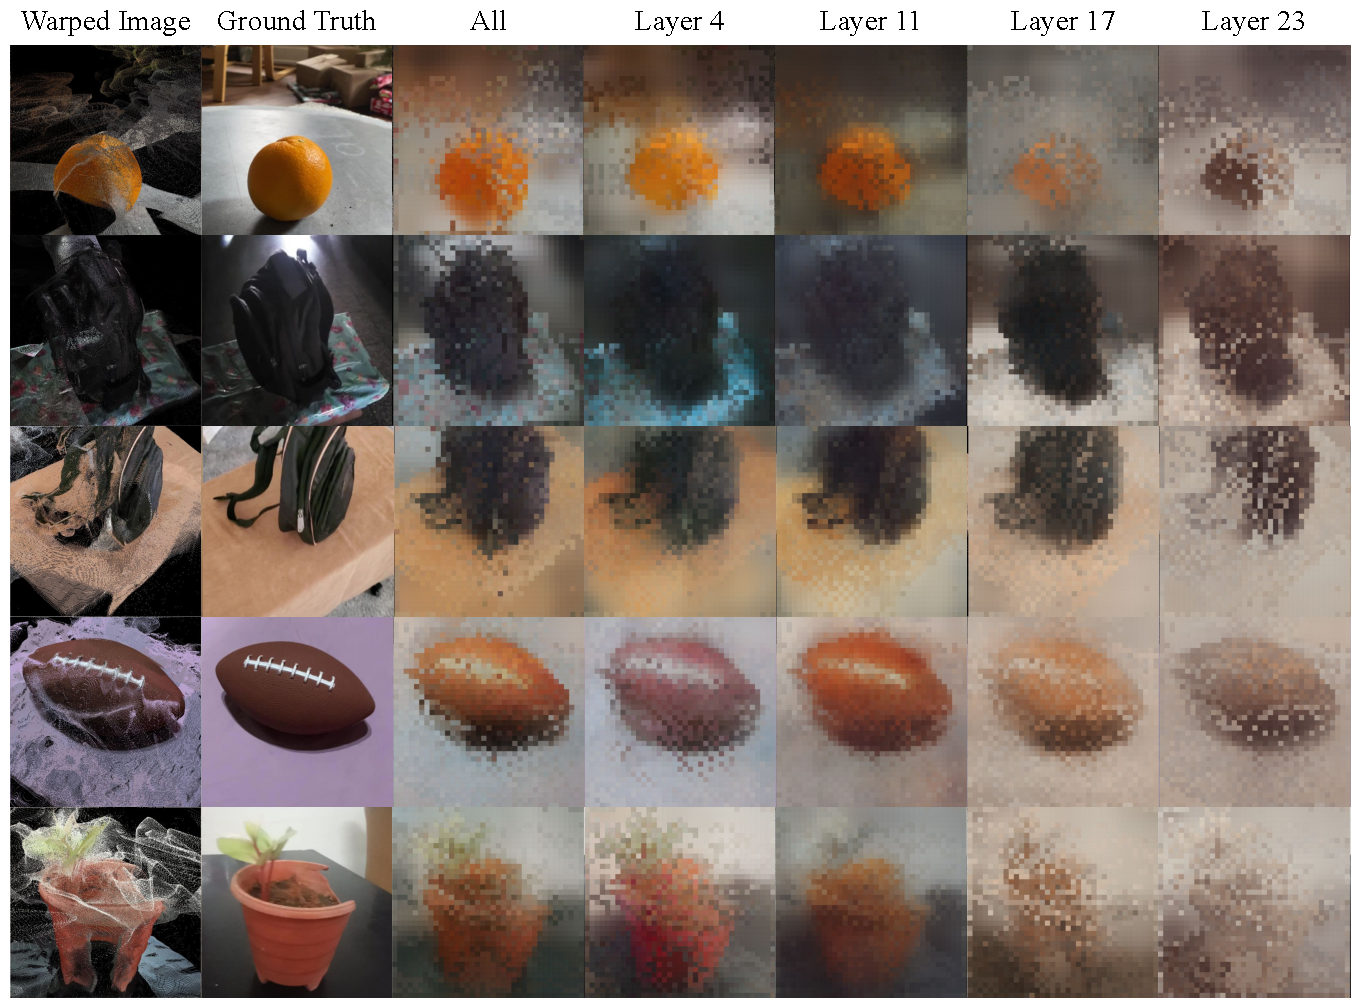
\includegraphics[width=1.0\linewidth]{Figures/appendix_recon_ablation_qual.pdf}
    \caption{\textbf{Per-layer probing qualitative results.} We visualize generation results using VGGT features extracted from individual layers and their combination. Early layers (4\textsuperscript{th}, 11\textsuperscript{th}) retain rich semantic information, producing semantically coherent images with accurate color and texture. In contrast, deeper layers (17\textsuperscript{th}, 23\textsuperscript{rd}) emphasize geometric structure but lack semantic detail. Combining features across all layers yields the most faithful reconstructions, achieving both structurally accurate and semantically realistic outputs.
    }
    \label{fig:appendix_recon_abl_qual}
    \vspace{-10pt}
\end{figure*}

\section{Additional Results}
\label{supp:exps}

% \subsection{Additional Comparison} 

% \begin{figure*}[t]
%     \centering
%     \includegraphics[width=1.0\linewidth]{Figures/Comparison_DTU.pdf}
%     \caption{\textbf{Qualitative comparison results.} Qualitative comparison against single-view warping-and-inpainting methods (LucidDreamer~\citep{chung2023luciddreamer}, GenWarp~\cite{seo2024genwarp}) on DTU dataset~\citep{jensen2014large}. All methods use VGGT~\cite{wang2025vggt} for geometry prediction. Our approach produces clean, geometrically consistent results while baseline methods exhibit visual artifacts and inconsistencies.}
%     \label{fig:appendix_dtu_qual}
%     \vspace{-10pt}
% \end{figure*}

% \begin{table}[t!]
% \begin{center}
% %\vspace{-20pt}
% \centering
%     \resizebox{0.5\textwidth}{!}{
%     \begin{tabular}{l|ccc}
%     \toprule
%           {\centering \textbf{Methods}} & PSNR$\uparrow$ & SSIM$\uparrow$ & LPIPS$\downarrow$ \\
%           \midrule
%           LucidDreamer~\cite{chung2023luciddreamer} & \textbf{12.96} & 0.248 & 0.385 \\
%           GenWarp~\cite{seo2024genwarp} & 8.69 & 0.253 & 0.597  \\
%           \textbf{ReNoV (Ours)} & 12.63 & \textbf{0.443} & \textbf{0.261} \\ 
%     \bottomrule
%     \end{tabular}}
%     \caption{\textbf{Comparison with other warping-and-inpainting models}. We compare our model against LucidDreamer~\cite{chung2023luciddreamer} (using SD-Inpainting~\cite{rombach2022high}) and GenWarp~\cite{seo2024genwarp}.} 
% \label{tab:comparison_quan}
% \vspace{-10pt}
% \end{center}
% \end{table}

% We compare our method against warping-and-inpainting approaches using single reference image, specifically LucidDreamer~\citep{chung2023luciddreamer} and GenWarp~\cite{seo2024genwarp}. Evaluation is conducted on the DTU dataset~\citep{jensen2014large}, which was excluded from training for all methods, thereby demonstrating zero-shot generalization capabilities. To ensure fair comparison, all warping-and-inpainting methods utilize VGGT~\cite{wang2025vggt} as the shared geometry prediction model. Quantitative results in Table~\ref{tab:comparison_quan} demonstrate that our framework achieves superior performance in SSIM and LPIPS, maintaining competitive results in PSNR. 

\subsection{Qualitative Results} 
Fig.~\ref{fig:qual_compare} presents qualitative comparisons on the RealEstate10k dataset. ReNoV w/ VGGT produces visually coherent reconstructions of the observed regions while plausibly extrapolating to unseen locations beyond the reference views. 
These results highlight the model’s ability to maintain spatial consistency and generate realistic scene content under view extrapolation.

Fig. \ref{fig:qual_dino_da3} provides a qualitative results of our framework integrated with diverse feature representations, using the same scenes from the DTU dataset shown in Fig.~\ref{fig:dtu_qual} for a direct comparison. Our method consistently yields high-fidelity synthesis that exceeds the baselines~\cite{charatan2024pixelsplat, chen2024mvsplat, ye2024no, zhang2025flare, jin2024lvsm}. Notably, while baselines frequently suffer from geometric distortions or blurring in unobserved areas, our framework maintains strict multi-view consistency. Furthermore, it demonstrates a superior capacity for generative inpainting, producing perceptually plausible textures sacrificing structural integrity.

\begin{figure*}[ht!]
    \centering
    \includegraphics[width=1.0\textwidth]{Figures/re10k_qual.pdf}
    \caption{\textbf{Qualitative comparison on RealEstate10k.} 
    Qualitative results demonstrate the extrapolative capability of our model (ReNoV w/ VGGT) to plausibly generate locations not seen in the reference images, while faithfully reconstructing the known regions. }
    \label{fig:qual_compare}
    \vspace{-10pt}
\end{figure*}

\begin{figure*}[ht!]
    \centering
    \includegraphics[width=1.0\textwidth]{Figures/qual_dino_da3.pdf}
    \caption{\textbf{Qualitative comparison of our framework across feature representations on DTU.} We visualize the robustness of our synthesis pipeline when utilizing different feature backbones, using the same scenes shown in Fig.~\ref{fig:dtu_qual}). Compared to state-of-the-art baselines, our method effectively mitigates structural artifacts and produces more coherent inpainting, regardless of the conditioning feature representation.
    }
    \label{fig:qual_dino_da3}
    \vspace{-10pt}
\end{figure*}



\subsection{Ablation Study}

\begin{figure*}[t]
    \centering
    \includegraphics[width=1.0\linewidth]{Figures/appendix_co3d_qual.pdf}
    \caption{\textbf{Qualitative ablation results.} (a) \textit{Baseline}: Lacks geometric guidance, resulting in misaligned structures (e.g., distorted chair, missing bicycle wheel, and incomplete teddy bear). (b) \textit{Baseline + pointmap}: Improves geometric alignment but suffers from distortion due to noisy geometry and inaccurate inpainting (e.g., deformed chair seat). (c) \textit{Ours with VGGT features}: Implicit semantic and geometric conditioning enables accurate reconstruction of visible regions and plausible inpainting of occluded areas.}
    \label{fig:appendix_co3d_qual}
    \vspace{-10pt}
\end{figure*}

\paragraph{Qualitative results.}
Fig.~\ref{fig:appendix_co3d_qual} shows additional ablation results for three configurations: (a) baseline with semantic-only conditioning; (b) baseline + explicit geometric guidance via pointmaps; (c) ours with implicit semantic and geometric conditioning using VGGT~\cite{wang2025vggt} features. Conditioning on VGGT features enables the model to achieve more accurate reconstructions and plausible inpainting by leveraging rich implicit geometric and semantic information. In contrast, (a) and (b) exhibit noticeable geometric distortions and incomplete inpainting, highlighting the limitations of lacking or noisy geometric cues.

% \begin{wrapfigure}{r}{0.6\textwidth}
%     \vspace{-20pt}
%     \centering
%     \includegraphics[width=1.0\linewidth]{Figures/appendix_attn_vis.pdf}
%     \caption{\textbf{Attention visualization for ablation study.} The leftmost column shows a query point (blue dot) in the warped image, with corresponding cross-attention maps over reference images shown on the right. Configurations (a) and (b) attend to incorrect regions for both reconstruction (e.g., teddy bear’s ear, bicycle handle) and inpainting (e.g., chair seat), due to limited or noisy geometric guidance. In contrast, VGGT-based conditioning (c) guides attention to geometrically and semantically aligned regions, accurately distinguishing fine structures such as the correct ear of the teddy bear.}
%     \label{fig:appendix_attn_vis}
%     \vspace{-20pt}
% \end{wrapfigure}

\paragraph{Attention map visualization.}
We further analyze the cross-view attention maps of the denoising U-Net trained under configurations (a), (b), and (c). As shown in Fig.~\ref{fig:appendix_attn_vis}, the baseline model (a) attends to geometrically and semantically misaligned regions in the reference images, leading to inaccurate reconstruction and inpainting. Explicit geometric guidance via pointmaps (b) partially reduces this misalignment but remains insufficient due to noisy and incomplete geometric correspondences. In contrast, our final model conditioned on VGGT~\cite{wang2025vggt} features (c) accurately attends to geometrically and semantically consistent regions in the reference views, significantly enhancing the quality of synthesized images. This confirms that VGGT features effectively guide cross-view attention toward optimal reference positions by implicitly encoding comprehensive geometric and semantic correspondences.

\begin{figure*}[t]
    \vspace{-20pt}
    \centering
    \includegraphics[width=0.8\linewidth]{Figures/appendix_attn_vis.pdf}
    \caption{\textbf{Attention map visualization for ablation study.} The leftmost column shows a query point (blue dot) in the warped image, with corresponding cross-attention maps over reference images shown on the right. Configurations (a) and (b) attend to incorrect regions for both reconstruction (e.g., teddy bear’s ear, bicycle handle) and inpainting (e.g., chair seat), due to limited or noisy geometric guidance. In contrast, VGGT-based conditioning (c) guides attention to geometrically and semantically aligned regions, accurately distinguishing fine structures such as the correct ear of the teddy bear.}
    \label{fig:appendix_attn_vis}
    \vspace{-10pt}
\end{figure*}

% \subsection{Architecture details}
% Our network architecture is composed of two primary streams: an image generation branch and a set of geometry prediction branches. The image generation branch employs a two-network design, where a reference network extracts detailed semantic features from input images, and a denoising U-Net synthesizes novel view images by leveraging aggregated multi-view attention. The reference network and the denoising U-Net are tightly coupled through a pointmap correspondence conditioning module that embeds 3D coordinates and a binary mask to provide explicit spatial alignment cues.

% On the geometry side, we employ three U-Nets with architectures identical to the image denoising network for predicting the depth map, pointmap, and normal map, respectively. To ensure cross-modal consistency, we incorporate cross-modal attention instillation by replacing the spatial attention maps of the geometry networks with those from the image denoising U-Net. This design choice not only regularizes the geometry prediction through deterministic training signals but also enhances the semantic richness of the geometric representations. Additionally, proximity-based mesh conditioning further refines the correspondence conditions, filtering out noisy projections and ensuring robust alignment between image and geometry synthesis.

% %%%%%%%%%%%%%%%%%%%%%%%%%%%%%%%%%%%%%%%%%%%%%%%%%%%%%%%%%%%%%%%%%%%%%%%%%%%%%%%

% \subsection{Depth prediction accuracy}
% We evaluate the depth prediction accuracy of our method using standard metrics such as PSNR, SSIM, and LPIPS. Quantitative comparisons against baseline methods demonstrate that our cross-modal attention instillation framework significantly reduces depth prediction error, particularly in challenging extrapolative scenarios. The integration of geometric cues via proximity-based mesh conditioning plays a critical role in refining the depth predictions, as evidenced by our ablation studies.

% In addition to the numerical evaluations, our qualitative assessments reveal that the depth maps generated by our approach exhibit smooth transitions and accurate handling of occluded regions. The enhanced structural consistency is directly attributable to the attention instillation mechanism, which transfers reliable spatial attention maps from the image domain to the geometry networks. These results underline the effectiveness of our method in achieving high-quality depth estimation that closely aligns with the ground-truth geometry.

% \begin{table*}[htb!]
%     \centering
%     \resizebox{\linewidth}{!}{%
%     \begin{tabular}{c|ccccc|ccccc}
%         \toprule
%         \multirow{2}{*}{\centering \textbf{Method}} & \multicolumn{5}{c|}{\textbf{Extrapolation}} & \multicolumn{5}{c}{\textbf{Interpolation}} \\
%         \cmidrule(lr){2-6} \cmidrule(lr){7-11}
%          & PSNR$\uparrow$ & SSIM$\uparrow$ & LPIPS$\downarrow$ & Abs.Rel$\downarrow$ & RMSE$\downarrow$
%          & PSNR$\uparrow$ & SSIM$\uparrow$ & LPIPS$\downarrow$ &
%          Abs.Rel$\downarrow$ & RMSE$\downarrow$\\
%         \midrule
%          PixelSplat~\cite{charatan2024pixelsplat}   
%          & 14.01 & 0.582 & 0.384 & 0.264 & 14.341 
%          & 23.85 & 0.806 & 0.185 & - & -  \\
%          MVSplat~\cite{chen2024mvsplat}  
%          & 12.13 & 0.534 & 0.380 & 0.234 & 13.986 
%          & 23.98 & 0.811 & 0.176 & - & - \\
%          NopoSplat~\cite{wu2023reconfusion}  
%          & 14.36 & 0.538 & 0.389 & 0.217 & 13.762
%          & \textbf{25.03} & \textbf{0.838} & \textbf{0.160} & - & -  \\
%         %  LucidDreamer~\cite{chung2023luciddreamer} 
%         %  & - & - & - & - & - 
%         %  & - & - & - & - & - \\
        
%         % GenWarp~\cite{seo2024genwarp} 
%         %  & - & - & - & - & - 
%         %  & - & - & - & - & - \\     
         
%          \midrule
%          \textbf{Ours} & \textbf{17.04} & \textbf{0.617} & \textbf{0.228} & \textbf{0.143} & \textbf{9.050}  & -- & -- & - & - & - \\
%         \bottomrule
%     \end{tabular}}
%     \caption{\textbf{Quantitative comparison of two-view 3D reconstruction}. Under the two-view setting, our method outperforms previous feedforward NVS approaches in the extrapolative setting in both image generation and depth prediction, while showing competitive performance in the interpolative setting as well.}
%     \label{tab:re10k}
%     \vspace{-10pt}
% \end{table*}
\clearpage
\newpage

% {\small
% \bibliographystyle{plain}
% \bibliography{main}
% }

% \end{document}